\section{Rengøring sidste dag}
\subsubsection*{\textbf{Ansvarlige:} \Randildo \& \Karla}

\begin{table}[H]
\centering
\begin{tabu}{l L{7cm} | L{4cm}}\specialrule{1pt}{0pt}{2pt}
\rowfont{\bfseries}
Hvor               & Hvem                 & Godkendt af \\ \specialrule{  1pt}{2pt}{1pt}
Køkkenet           & \Buddha Buddhisterne &             \\ \specialrule{.25pt}{1pt}{1pt}
Soveværelser       & \Hemorides Grækkerne &             \\ \specialrule{.25pt}{1pt}{1pt}
Sal foran køkkenet & \Clint 'Murica       &             \\ \specialrule{.25pt}{1pt}{1pt}
Spisesal/Musik     & \Stive Australien    &             \\ \specialrule{.25pt}{1pt}{1pt}
Pejsestuen/Øl      & \Mighty Skotland     &             \\ \specialrule{.25pt}{1pt}{1pt}
Gange              & \Randildo Brasilien  &             \\ \specialrule{.25pt}{1pt}{1pt}
Toiletter/Baderum  & \Farav Ægypten       &             \\ \specialrule{.25pt}{1pt}{1pt}
Udendørsområder    & \Karla Vikingerne    &             \\ \specialrule{  1pt}{1pt}{1pt}
\end{tabu}
\end{table}

\subsection*{Rengøringsplan - Afskrevet fra lejekontrakt}
Alle gulve fejes og vaskes og overflader tørres af med en våd klud. Gulvtæpper støvsuges. Fryser og køleskab slukkes og afvaskes. Service sættes på plads. Toiletter, baderum og håndvaske rengøres grundigt. Udendørsarealer rengøres for affald. Kongressen er rengjort og lukket allerede om torsdagen.\\
Alt bagage lægges i gården.\\
Vi skal anmelde og erstatte manglende eller ødelagt service og inventar. Anmeldese påføres rapport, som kan findes i holderen i køkkenet, og som ved afrejsen efterlades på køkkenbordet. 

%\begin{figure}[H]
%\begin{center}
%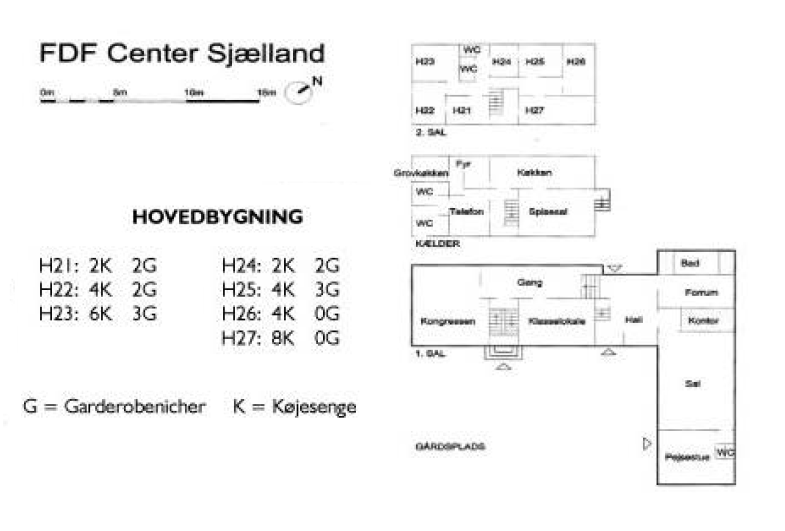
\includegraphics[height=5cm]{fig/Grundplan.png}
%\caption{Plan over Center Sjælland}
%\end{center}
%\end{figure}